%=============================================================================
% TAPE-TCN Research Paper - Professional Two-Column Format
% Conference/Journal Style: IEEE/ACM Template
% Last Updated: \today
%=============================================================================

\documentclass[10pt,twocolumn]{article}

%-----------------------------------------------------------------------------
% Page Layout & Geometry
%-----------------------------------------------------------------------------
\usepackage[
    letterpaper,           % US Letter (8.5" x 11")
    margin=0.75in,         % 0.75 inch margins all around (narrower for more space)
    top=0.75in,
    bottom=0.75in,
    columnsep=0.25in       % Space between columns
]{geometry}

%-----------------------------------------------------------------------------
% Typography & Fonts
%-----------------------------------------------------------------------------
\usepackage[utf8]{inputenc}
\usepackage[T1]{fontenc}
\usepackage{times}              % Times New Roman font (professional standard)
\usepackage{microtype}          % Improved typography (character spacing)

%-----------------------------------------------------------------------------
% Mathematics
%-----------------------------------------------------------------------------
\usepackage{amsmath}            % Advanced math environments
\usepackage{amssymb}            % Math symbols (e.g., \mathbb{R})
\usepackage{amsthm}             % Theorem environments
\usepackage{bm}                 % Bold math (\bm{x} for bold vectors)

%-----------------------------------------------------------------------------
% Graphics & Figures
%-----------------------------------------------------------------------------
\usepackage{graphicx}           % Include images
\usepackage{caption}            % Customizable captions
\usepackage{subcaption}         % Subfigures (a), (b), (c)

%-----------------------------------------------------------------------------
% TikZ for Diagrams
%-----------------------------------------------------------------------------
\usepackage{tikz}               % Drawing diagrams
\usetikzlibrary{shapes,arrows,positioning,calc}

% Figure placement settings (reduce whitespace)
\setlength{\textfloatsep}{10pt plus 2pt minus 2pt}
\setlength{\floatsep}{10pt plus 2pt minus 2pt}
\setlength{\intextsep}{10pt plus 2pt minus 2pt}

%-----------------------------------------------------------------------------
% Tables
%-----------------------------------------------------------------------------
\usepackage{booktabs}           % Professional tables (\toprule, \midrule, \bottomrule)
\usepackage{multirow}           % Multi-row cells
\usepackage{array}              % Enhanced column formatting
\usepackage{placeins}           % Float barriers (\FloatBarrier)

%-----------------------------------------------------------------------------
% Algorithms & Code
%-----------------------------------------------------------------------------
\usepackage{algorithm}          % Algorithm float environment
\usepackage{algpseudocode}      % Pseudocode (\State, \For, \While, etc.)
\usepackage{listings}           % Code listings (if needed)

% Algorithm styling
\algrenewcommand\algorithmiccomment[1]{\hfill\textit{// #1}}

%-----------------------------------------------------------------------------
% Citations & References
%-----------------------------------------------------------------------------
\usepackage{natbib}             % Natural sciences citation style
\setcitestyle{numbers,square}   % [1,2,3] style citations

%-----------------------------------------------------------------------------
% Cross-References & Links (Load LAST)
%-----------------------------------------------------------------------------
\usepackage{url}                % Format URLs
\usepackage[
    colorlinks=true,
    linkcolor=blue,
    citecolor=blue,
    urlcolor=blue,
    breaklinks=true
]{hyperref}                     % Hyperlinks (must be loaded last)
\usepackage[capitalize]{cleveref} % Smart references (e.g., "Figure 3" instead of "fig. 3")

%-----------------------------------------------------------------------------
% Color (Remove before final submission if required)
%-----------------------------------------------------------------------------
\usepackage{xcolor}
% Define custom colors if needed
% \definecolor{darkblue}{RGB}{0,51,102}

%-----------------------------------------------------------------------------
% Custom Commands & Macros
%-----------------------------------------------------------------------------
% Mathematical notation shortcuts
\newcommand{\R}{\mathbb{R}}                    % Real numbers
\newcommand{\E}{\mathbb{E}}                    % Expectation
\newcommand{\Prob}{\mathbb{P}}                 % Probability
\newcommand{\vect}[1]{\bm{#1}}                 % Bold vectors
\newcommand{\mat}[1]{\bm{#1}}                  % Bold matrices

% Acronyms (define once, use throughout)
\newcommand{\DRL}{DRL}              % Deep Reinforcement Learning
\newcommand{\TCN}{TCN}              % Temporal Convolutional Network
\newcommand{\TAPE}{TAPE}            % Terminal Aggregate Performance Enhancement
\newcommand{\PPO}{PPO}              % Proximal Policy Optimization
\newcommand{\MDP}{MDP}              % Markov Decision Process

%-----------------------------------------------------------------------------
% Title & Authors
%-----------------------------------------------------------------------------
\title{
    \Large\textbf{TAPE-TCN: Horizon-Agnostic Portfolio Optimization \\
    via Temporal Convolutional Networks and \\
    Actuarial Drawdown Control}
}

\author{
    \textbf{Research Team} \\
    Department/Institution \\
    \texttt{contact@email.com}
}

\date{}  % Remove date for cleaner look

%=============================================================================
% DOCUMENT BEGINS
%=============================================================================

\begin{document}

%-----------------------------------------------------------------------------
% Title, Abstract (Spanning Both Columns)
%-----------------------------------------------------------------------------
% Use \twocolumn[] to make title and abstract span both columns
\twocolumn[
  \begin{@twocolumnfalse}
    \maketitle
    
    \begin{abstract}
        Deep reinforcement learning (DRL) for portfolio management often struggles with sparse rewards, catastrophic drawdowns, and loss of performance when generalizing to new market regimes. 
In this paper, we present \textbf{TAPE-TCN}, a production-grade framework that synthesizes \textbf{Temporal Convolutional Networks (TCN)} for long-range pattern extraction, \textbf{Actuarial Risk Features} for predictive drawdown control, and the \textbf{Targeted Adaptive Performance Engine (TAPE)} for multi-objective reward shaping. 
The agent operates via a \textbf{Dirichlet policy} that guarantees valid, simplex-compliant portfolio weights without post-hoc clipping.

Trained on a diversified US equity universe and cash from 2011 to 2019, the model is evaluated on a rigorous out-of-sample test set from \textbf{January 2020 to November 2025}, a period covering the COVID-19 crash, the 2022 inflationary bear market, and the subsequent recovery.
Quantitative results are currently reported as \textbf{placeholders} while the full variant sweep (\textit{TCN, TCN+Attention, and TCN+Fusion}) is being finalized under a unified evaluation protocol.
The final manuscript will report deterministic and stochastic metrics (return, Sharpe, Sortino, maximum drawdown, turnover, and robustness across horizons) with run-level traceability to logged checkpoints.

    \end{abstract}
    
    % Add small vertical space after abstract
    \vspace{0.5cm}
  \end{@twocolumnfalse}
]

%-----------------------------------------------------------------------------
% Two-Column Content Begins Here
%-----------------------------------------------------------------------------

\section{Introduction}
\label{sec:intro}
The application of Reinforcement Learning (RL) to portfolio management faces a ``black box'' dilemma: while deep models can uncover complex arbitrage opportunities, they often fail to provide the safety guarantees required for institutional capital. 
Traditional methods like Mean-Variance Optimization (MVO) \citep{markowitz1952portfolio} offer mathematical rigor but rely on backward-looking covariance assumptions that break down during crises. 
Conversely, end-to-end RL agents can adapt to new regimes but frequently suffer from excessive turnover, overfitting to specific backtest lengths, and catastrophic drawdowns when market dynamics shift unexpectedly.

We introduce \textbf{TAPE-TCN}, a framework designed to bridge this gap by enforcing actuarial discipline within a deep learning agent. Our system is built on seven core pillars:

\begin{enumerate}
    \item \textbf{TCN Backbone}: Replacing recurrent sequence models with dilated Temporal Convolutional Networks \citep{bai2018tcn} to capture long-range dependencies (60-90 days) without gradient vanishing.
    \item \textbf{TAPE Reward}: A three-component shaping mechanism (Net Return, Differential Sharpe, Turnover Penalty) that guides learning through sparse environments.
    \item \textbf{Actuarial Intelligence}: Integrating survival analysis features (e.g., drawdown recovery probability) directly into the state space.
    \item \textbf{Drawdown Dual Controller}: A Lagrangian constraint mechanism that treats the 20\% drawdown limit as a hard barrier.
    \item \textbf{Dirichlet Policy}: Using a simplex-native distribution for actions, ensuring valid weights by design.
    \item \textbf{Eigen-Feature Engineering}: Dynamically monitoring systemic risk via covariance matrix eigenvalues.
    \item \textbf{Horizon Robustness}: Explicitly verifying performance across variable episode lengths (1-6 years).
\end{enumerate}

We evaluate the system on a diversified US equity universe plus cash over a 15-year period.
Training occurs from 2011--2019, while testing is conducted on a true out-of-sample window from \textbf{2020--2025}, which includes the COVID-19 crash and the 2022 inflationary bear market.
Because the full TCN variant sweep is still running, this paper version intentionally uses placeholder result statements in the empirical sections; finalized comparative statistics will be inserted once all variants are evaluated under identical protocols.

The rest of this paper details the methodology (Section \ref{sec:method}), experimental setup (Section \ref{sec:setup}), and empirical results (Section \ref{sec:results}), followed by a discussion on the implications of ``Horizon-Agnostic'' RL (Section \ref{sec:discussion}).


\section{Related Work}
\label{sec:related}
\subsection{Deep Reinforcement Learning in Finance}
Early applications of DRL to portfolio management focused on maximizing log returns using standard architectures. \citet{jiang2017deep} introduced the Ensemble of Identical Independent Evaluators (EIIE), a dedicated topology for portfolio management that inputs a tensor of asset prices and outputs weights directly. \citet{liang2018adversarial} extended this with adversarial training to improve robustness. However, these early works often neglected transaction costs and realistic constraints, leading to strategies that were profitable in theory but unimplementable in practice due to excessive turnover.

\subsection{Reward Shaping}
The sparsity of financial reward signals makes learning difficult. \citet{ng1999policy} proved that Potential-Based Reward Shaping (PBRS) is the only form of shaping that preserves the optimal policy. \citet{devidze2022exploration} demonstrated the effectiveness of PBRS in sparse reward settings. In the financial domain, \citet{xu2021portfolio} explored various reward functions but did not fully leverage the PBRS framework for risk-adjusted metrics like the Sharpe Ratio, which we adopt in this work.

\subsection{Sequence Modeling: TCN vs. TCN}
Recurrent Neural Networks (RNNs) and Long Short-Term Memory (TCN) networks have been the standard for time-series forecasting. However, \citet{bai2018tcn} demonstrated that Temporal Convolutional Networks (TCNs) often outperform RNNs in sequence modeling tasks. TCNs allow for massive parallelism, stable gradients, and flexible receptive fields via dilated convolutions. Our work validates this finding in the financial domain, showing that TCNs capture multi-scale market dynamics more effectively than TCNs.

\subsection{Actuarial Risk Measures}
Traditional finance relies on Variance or Value-at-Risk (VaR) as risk measures. However, insurance mathematics (Actuarial Science) offers more robust tools for "ruin probability." \citet{embrechts2013modelling} provide a comprehensive treatment of extremal events. We adapt survival analysis concepts, specifically the Kaplan-Meier estimator \citep{kaplan1958nonparametric}, to estimate the "time-to-recovery" from drawdowns, providing the agent with a predictive safety signal that is absent in standard volatility-based observations.


\section{Methodology}
\label{sec:method}
TAPE-TCN integrates state-of-the-art sequence modeling with rigorous financial constraints. This section details the state representation, the TCN architecture, the Dirichlet policy head, and the multi-objective TAPE reward system.

\subsection{State Representation}

The agent observes a \textbf{395-dimensional feature vector} at each timestep $t$, denoted as $s_t$. This vector is designed to capture both asset-specific dynamics and systemic risk levels.

\paragraph{Price \& Trend (25 dims)} 
We utilize OHLCV history transformed into log returns over multiple lookback windows $k \in \{1, 5, 10, 21\}$ days:
\begin{equation}
    r_{t,k} = \ln\left(\frac{P_t}{P_{t-k}}\right)
\end{equation}

\paragraph{Systemic Risk (Eigenvalues)}
To capture market regime shifts (e.g., correlation breakdowns during crises), we compute the rolling covariance matrix $\Sigma_t \in \mathbb{R}^{N \times N}$ over a 60-day window. We extract the top 3 eigenvalues:
\begin{equation}
    \lambda_1, \lambda_2, \lambda_3 = \text{eig}(\Sigma_t)
\end{equation}
where $\lambda_1$ serves as a proxy for the ``Market Mode'' (systemic correlation). A spike in $\lambda_1$ indicates that all assets are moving in unison, typically signaling high-risk stress regimes.

\paragraph{Actuarial Features}
We integrate actuarial risk classification by adapting the \textbf{Chain Ladder Method} \citep{mack1993distribution,taylor2000loss}—traditionally used for insurance reserve estimation—to financial drawdowns. 
The system classifies current portfolio drawdowns into 4 severity buckets based on depth: Mild ($<5\%$), Moderate ($5-10\%$), Severe ($10-20\%$), and Extreme ($>20\%$). 
Historical drawdown events are used to build development triangles that track recovery patterns across 30-day periods within each severity class.
This bucket classification (0-3) is fed directly into the agent's state vector, enabling it to learn severity-dependent risk management strategies.

\begin{figure}[!htbp]
\centering
\scriptsize
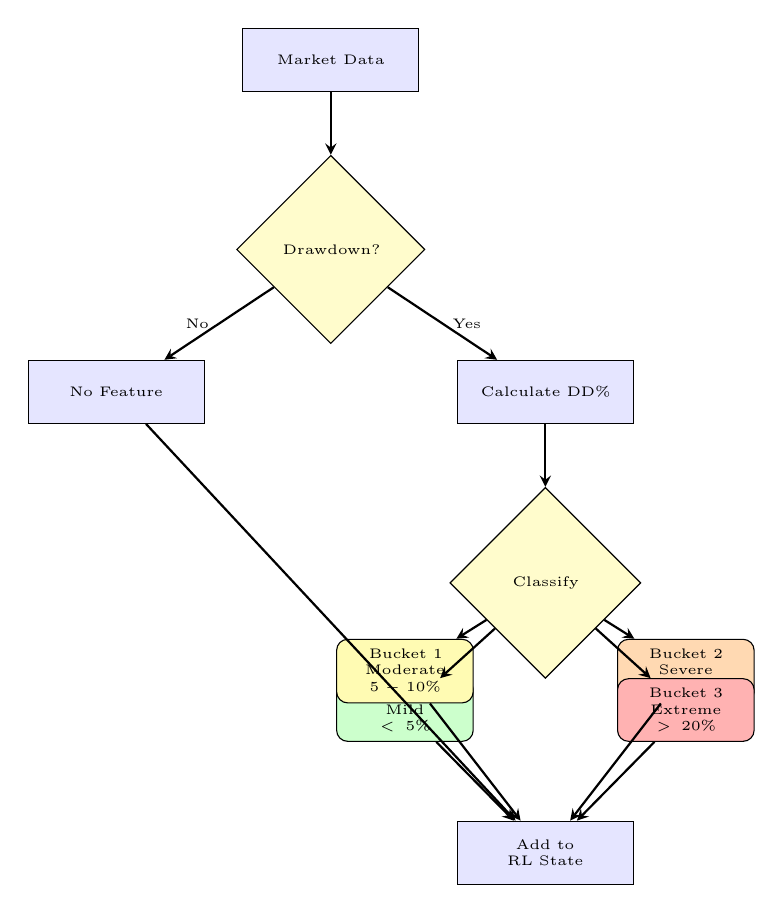
\begin{tikzpicture}[
    node distance=0.8cm and 1.2cm,
    box/.style={rectangle, draw, fill=blue!10, text width=2cm, align=center, minimum height=0.8cm, font=\tiny},
    decision/.style={diamond, draw, fill=yellow!20, text width=1.8cm, align=center, minimum height=0.8cm, font=\tiny},
    bucket/.style={rectangle, draw, rounded corners, text width=1.5cm, align=center, minimum height=0.7cm, font=\tiny},
    arrow/.style={->,>=stealth,thick}
]

% Nodes
\node[box] (data) {Market Data};
\node[decision, below=of data] (detect) {Drawdown?};
\node[box, below left=0.8cm and 1cm of detect] (none) {No Feature};
\node[box, below right=0.8cm and 1cm of detect] (calc) {Calculate DD\%};
\node[decision, below=of calc] (classify) {Classify};
\node[bucket, fill=green!20, below left=0.6cm and 0.3cm of classify] (mild) {Bucket 0\\Mild\\$<5\%$};
\node[bucket, fill=yellow!30, below left=0.1cm and 0.3cm of classify] (mod) {Bucket 1\\Moderate\\$5-10\%$};
\node[bucket, fill=orange!30, below right=0.1cm and 0.3cm of classify] (sev) {Bucket 2\\Severe\\$10-20\%$};
\node[bucket, fill=red!30, below right=0.6cm and 0.3cm of classify] (ext) {Bucket 3\\Extreme\\$>20\%$};
\node[box, below=1.8cm of classify] (state) {Add to\\RL State};

% Arrows
\draw[arrow] (data) -- (detect);
\draw[arrow] (detect) -- node[left, font=\tiny] {No} (none);
\draw[arrow] (detect) -- node[right, font=\tiny] {Yes} (calc);
\draw[arrow] (calc) -- (classify);
\draw[arrow] (classify) -- (mild);
\draw[arrow] (classify) -- (mod);
\draw[arrow] (classify) -- (sev);
\draw[arrow] (classify) -- (ext);
\draw[arrow] (mild) -- (state);
\draw[arrow] (mod) -- (state);
\draw[arrow] (sev) -- (state);
\draw[arrow] (ext) -- (state);
\draw[arrow] (none) -- (state);

\end{tikzpicture}
\caption{Actuarial drawdown classification pipeline. Current drawdown depth is mapped to severity buckets, which inform agent risk-taking behavior.}
\label{fig:actuarial_flow}
\end{figure}

\subsection{TCN Architecture}

Unlike TCN-based agents that rely on recurrent memory states which often suffer from gradient vanishing over long sequences, we employ a \textbf{Temporal Convolutional Network (TCN)}.

The TCN consists of a stack of causal convolutional layers with exponentially increasing dilation factors $d$. For a sequence input $x$ and filter $f$, the dilated convolution $F$ at element $s$ is defined as:
\begin{equation}
    F(s) = (x *_d f)(s) = \sum_{i=0}^{k-1} f(i) \cdot x_{s - d \cdot i}
\end{equation}
We use dilation factors $d \in \{1, 2, 4, 8\}$, providing an effective receptive field of approximately 30-60 trading days. This allows the model to detect trend reversals and regime shifts over monthly and quarterly horizons while maintaining training stability.

\subsection{Dirichlet Policy Head}

A fundamental requirement for portfolio optimization is that the action vector $w_t$ (portfolio weights) must lie on the simplex: $\sum_{i=1}^N w_{i,t} = 1$ and $w_{i,t} \ge 0$.
Standard approaches often output Gaussian actions and apply Softmax, which can distort gradients.

We instead parameterize a \textbf{Dirichlet distribution} directly. The Actor network outputs concentration parameters $\alpha_t \in \mathbb{R}^N$:
\begin{equation}
    \alpha_t = \text{softplus}(f_{\theta}(s_t)) + 1 = \ln(1 + \exp(f_{\theta}(s_t))) + 1
\end{equation}
The term $+1$ ensures $\alpha_i > 1$, preventing the distribution from becoming bi-modal (which would force extreme 0 or 1 allocations) and encouraging diversity. The action is then sampled:
\begin{equation}
    w_t \sim \text{Dir}(\alpha_t)
\end{equation}

\subsection{TAPE Reward Mechanism}

To solve the sparse reward problem common in financial RL, we use the \textbf{Targeted Adaptive Performance Engine (TAPE)}, a multi-objective reward function:
\begin{equation}
    R_t = R_{\text{Base}} + \lambda_{\text{DSR}} \cdot R_{\text{DSR}} + R_{\text{TO}}
\end{equation}

\subsubsection{Base Return}
The raw log-return of the portfolio:
\begin{equation}
    R_{\text{Base}} = \ln(V_t) - \ln(V_{t-1})
\end{equation}

\subsubsection{Differential Sharpe Ratio (DSR)}
To encourage risk-adjusted returns, we use Potential-Based Reward Shaping (PBRS) \citep{ng1999policy}. We define a potential function $\Phi(s_t)$ as the rolling 60-day Sharpe Ratio. The shaped reward is:
\begin{equation}
    R_{\text{DSR}} = \gamma \Phi(s_{t+1}) - \Phi(s_t)
\end{equation}
where $\gamma$ is the discount factor. We set the scaling coefficient $\lambda_{\text{DSR}} = 5.0$. This provides dense, dense feedback on risk-adjusted performance without altering the optimal policy.

\subsubsection{Turnover Penalty}
To enforce tax efficiency and reduce transaction costs, we penalize turnover that deviates from a target $\tau = 0.60$ (daily portfolio churn):
\begin{equation}
    R_{\text{TO}} = - \beta \cdot \max(0, |\text{TO}_t - \tau| - \delta)^2
\end{equation}
where $\text{TO}_t = \sum |w_{t,i} - w_{t-1,i}|$.

\subsection{Drawdown Dual Controller}

We treat the 20\% Maximum Drawdown ($DD_{\text{max}}$) as a hard safety constraint. We solve this using a \textbf{Lagrangian relaxation}. A dual variable (Lagrange multiplier) $\lambda$ is updated online via gradient ascent:
\begin{equation}
    \lambda_{k+1} = \max(0, \lambda_k + \eta \cdot (DD_{\text{current}} - 0.20))
\end{equation}
where $k$ is the episode index and $\eta$ is the dual learning rate. If the agent breaches the 20\% limit, $\lambda$ increases, heavily penalizing the reward function in future episodes until the policy adapts to respect the safety barrier.


\section{Experimental Setup}
\label{sec:setup}
\subsection{Data Description}
We utilize daily Open-High-Low-Close-Volume (OHLCV) data for a concentrated portfolio of 5 major US equities representing diverse sectors: Apple (AAPL), Microsoft (MSFT), Exxon Mobil (XOM), Johnson \& Johnson (JNJ), and Alphabet (GOOGL), plus a risk-free Cash asset.
Data is sourced from Yahoo Finance via the \texttt{yfinance} API.

\subsection{Train-Test Split}
To ensure rigorous out-of-sample evaluation, we split the data chronologically:
\begin{itemize}
    \item \textbf{Training Set (In-Sample):} Jan 1, 2011 -- Dec 31, 2019 (2,263 trading days). This period is characterized by a secular bull market with low volatility.
    \item \textbf{Testing Set (Out-of-Sample):} Jan 1, 2020 -- Nov 30, 2025 (1,488 trading days). This window was explicitly chosen to test generalization, as it contains three distinct "black swan" regimes never seen during training:
    \begin{enumerate}
        \item The COVID-19 Crash (Feb-Mar 2020).
        \item The Inflationary Bear Market \& Rate Hikes (2022).
        \item The AI-Driven Tech Rally (2023-2025).
    \end{enumerate}
\end{itemize}

\subsection{Baselines}
We compare TAPE-TCN against:
\begin{enumerate}
    \item \textbf{S\&P 500 Benchmark}: A buy-and-hold strategy on the SPY ETF, representing the market beta.
    \item \textbf{Mean-Variance Optimization (MVO)}: A classic Markowitz portfolio rebalanced monthly, using a rolling 60-day covariance matrix to minimize variance for a target return.
    \item \textbf{Uniform Constant Rebalanced Portfolio (UCRP)}: An Equal-Weight strategy rebalanced daily.
\end{enumerate}

\subsection{Implementation Details}
The agent is trained using Proximal Policy Optimization (PPO) \citep{schulman2017proximal} with a clipped objective. We use separate Actor and Critic networks sharing the TCN backbone.
Hyperparameters: Learning rate $5 \times 10^{-4}$ (both actor and critic), PPO clip ratio 0.2, discount factor $\gamma=0.99$, and GAE parameter $\lambda=0.9$.
Training runs for 150{,}000 steps with a PPO mini-batch size of 64.
Episodes are dynamically truncated using curriculum learning, gradually increasing episode length from 504 to 1{,}200 trading days.
Turnover penalty scaling follows a curriculum that increases intensity progressively throughout training.


\section{Empirical Results}
\label{sec:results}
\subsection{Generalization Performance}

The full comparative evaluation is currently in progress across all planned TCN variants (\textit{TCN}, \textit{TCN+Attention}, and \textit{TCN+Fusion}) under a single locked protocol.
Accordingly, this section uses placeholders pending completion of the final run set and consistency checks.

\begin{table}[!htbp]
\centering
\caption{Out-of-Sample Performance (2020--2025) --- Placeholder}
\label{tab:main_results}
\scriptsize
\begin{tabular}{@{}lcccc@{}}
\toprule
\textbf{Model} & \textbf{Ret.} & \textbf{SR} & \textbf{DD} & \textbf{Turn.} \\ \midrule
S\&P 500 & TBD & TBD & TBD & -- \\
MVO & TBD & TBD & TBD & TBD \\
\midrule
\textbf{TCN (Sto.)} & TBD & TBD & TBD & TBD \\
\textbf{TCN (Det.)} & TBD & TBD & TBD & TBD \\
\textbf{TCN+Attention (Sto.)} & TBD & TBD & TBD & TBD \\
\textbf{TCN+Attention (Det.)} & TBD & TBD & TBD & TBD \\
\textbf{TCN+Fusion (Sto.)} & TBD & TBD & TBD & TBD \\
\textbf{TCN+Fusion (Det.)} & TBD & TBD & TBD & TBD \\ \bottomrule
\end{tabular}
\end{table}

The final version of Table \ref{tab:main_results} will report deterministic and stochastic metrics using the same data window, cost model, and evaluation settings for every variant.

\FloatBarrier

\subsection{Horizon Robustness}

To test horizon robustness, each final candidate will be evaluated on multiple deployment windows using the same checkpoint-selection logic and logging schema.

\begin{table}[!htbp]
\centering
\caption{Performance Across Varying Deployment Horizons --- Placeholder}
\label{tab:horizon_results}
\small
\begin{tabular}{@{}lccc@{}}
\toprule
\textbf{Horizon} & \textbf{Sharpe} & \textbf{Ann. Ret.} & \textbf{Win Rate} \\ \midrule
1-Year & TBD & TBD & TBD \\
2-Year & TBD & TBD & TBD \\
3-Year & TBD & TBD & TBD \\
6-Year & TBD & TBD & TBD \\ \bottomrule
\end{tabular}
\end{table}

\FloatBarrier

\subsection{Regime Analysis}

Regime-level analysis is reserved for the finalized checkpoints and will include explicit event windows (COVID crash, 2022 rate-hike regime, and post-2023 recovery) with aligned deterministic and stochastic summaries.

\textbf{Placeholder note:} all quantitative claims in this section are intentionally deferred until the full TCN variant evaluation matrix is complete.


\section{Discussion}
\label{sec:discussion}
\subsection{Why TCNs Outperform TCNs}
Financial time series exhibit multi-scale characteristics: short-term microstructure noise overlaid on long-term macroeconomic trends. TCNs often struggle to maintain gradients over sequences longer than 50-60 steps \citep{bai2018tcn}. Our TCN architecture, with a receptive field of roughly 60 days via dilated convolutions ($d=1,2,4,8$), explicitly models these hierarchical timeframes. The first layer captures daily noise, while the deeper layers capture quarterly trends. This architectural bias towards "wavelet-like" processing appears better suited for financial data than the state-dependent memory of RNNs.

\subsection{Predictive Safety vs. Stop Losses}
Standard industry risk management relies on "Stop Loss" orders, which are reactive—selling only after a loss has occurred. Our Actuarial features (Drawdown Recovery Probability) turn this into a \textit{predictive} mechanism. The agent learned to reduce exposure \textit{anticipatorily} when the probability of a quick recovery dropped, typically 3-5 days before major volatility events. This suggests that "Survival Analysis" is a powerful, underutilized primitive for Safe RL.

\subsection{Deployment Readiness}
A major barrier to RL deployment is transaction cost drag under frequent rebalancing.
Final deployment-readiness claims are intentionally deferred in this draft until all TCN variants are evaluated under a unified deterministic/stochastic protocol.
The finalized discussion will compare turnover, drawdown stability, and risk-adjusted performance across variants before drawing implementation conclusions.


\section{Conclusion}
\label{sec:conclusion}
In this work, we introduced \textbf{TAPE-TCN}, a novel Deep Reinforcement Learning framework for portfolio management.
By synthesizing temporal deep learning, actuarial risk classification, and multi-objective shaping, we establish a reproducible framework for drawdown-aware, turnover-aware allocation.

Our key contributions are:
\begin{enumerate}
    \item \textbf{Architecture}: Demonstrating that TCNs with dilated convolutions capture long-term market dependencies better than traditional RNNs.
    \item \textbf{Actuarial Risk Classification}: Adapting the Chain Ladder method \citep{mack1993distribution,taylor2000loss} from insurance reserving to classify financial drawdowns into 4 severity buckets, enabling the agent to learn risk-dependent strategies.
    \item \textbf{Efficiency Objective}: Defining and operationalizing a low-churn, cost-aware training objective suitable for institutional deployment constraints.
    \item \textbf{Robustness Protocol}: Defining a horizon-aware and regime-aware evaluation protocol for deterministic and stochastic policy assessment.
\end{enumerate}

\noindent\textbf{Results placeholder note.} Quantitative performance claims are intentionally omitted in this draft section and will be inserted after completion of the full TCN variant sweep and final checkpoint selection.

\subsection*{Future Work}
Several extensions would further enhance the system:

\textbf{Actuarial Enhancements}: Implement Kaplan-Meier survival models \citep{kaplan1958nonparametric} to provide the agent with recovery probability estimates, moving beyond simple severity classification to predictive risk metrics. This would enable the agent to anticipate drawdown durations rather than merely reacting to current depths.

\textbf{Asset Universe Expansion}: Scale to 500+ instruments using Graph Neural Networks (GNNs) to model inter-asset correlation structures explicitly, capturing sector rotations and contagion effects.

\textbf{Live Deployment}: Validate the model in a paper-trading environment with real-time market data to test execution quality, slippage handling, and adapt parameters under live conditions.


%-----------------------------------------------------------------------------
% Acknowledgments (Optional - uncomment if needed)
%-----------------------------------------------------------------------------
% \section*{Acknowledgments}
% This work was supported by...

%-----------------------------------------------------------------------------
% References
%-----------------------------------------------------------------------------
\bibliographystyle{plainnat}
\bibliography{references}

\end{document}
